\documentclass[../Analysis-3]{subfiles}

\begin{document}
\chapter*{Lecture 25} %Set chapter name
\addcontentsline{toc}{chapter}{Lecture 25} %Set chapter title
\setcounter{chapter}{25} %Set chapter counter
\setcounter{section}{0}
%The content
\section{Tangent Plane Of $\mathcal{G}(f)$}

Let, $f : \mathcal{O}_2 \to \R$ be a $C^1$ function and $r(u,v) = (u,v,f(u,v))$. Here $\text{ran}(r)$ defines a surface $\mathcal{G}(f)$ as we have showed in $\ref{eg:grp}$. We also have calculated $r_v\times r_u = (-f_u,-f_v,1)$. Now using $\ref{eq:4}$ we can write down the equation of \textbf{Tangent space} at a point $P = (a,b,f(a,b))$ on $\mathcal{G}(f)$. Equation of the tangent space $T_P \mathcal{S}$

\begin{align}\label{eq:tp}
    f_u(a,b)(x-a) + f_v(a,b)(y-b)-(z-f(a,b))         & = 0 \\
    \implies z = f(a,b) + f_u(a,b)(x-a) + f_v(a,b)(y & -b)
\end{align}

Equation of \textbf{Normal} at the point $P$ on the surface $\mathcal{G}(f)$ is,
\begin{align}\label{eq:np}
    \frac{x-a}{-f_u(a,b)} = \frac{y-b}{-f_v(a,b)} = \frac{z-f(a,b)}{1}
\end{align}

\begin{Eg}{Equation of Tangent and Normal to $z = f(x,y) = \frac{2x}{y}-y^2$ at $(1,1,1)$}{}
    \textit{Solution.} This is a graph function so obviously a surface $f_x(x,y) = \frac{2}{y}$ and $f_y = -\frac{2x}{y^2} -2y$. So,$\langle -f_x,- f_y,1 \rangle = \langle -2,4,1\rangle$. So equation of Normal
    is $\frac{x-1}{-2}=\frac{y-1}{4}=\frac{z-1}{1}$ and the equation of Tangent Plane is,
    $ 2(x-1)-4(y-1) -(z-1) = 0$. $\hfill \blacksquare $
\end{Eg}
\begin{Eg}{Use Tangent Plane to approximate $(1.99)^2 - \frac{1.99}{1.01}$}{}
    \textit{Solution.} Consider $z = x^2 - \frac{x}{y} = f(x,y)$. This describes a surface. Now consider $P=(2,1,2)$ be the point on the surface. Here,$\langle -f_x,- f_y,1 \rangle = \langle -3,-2,1\rangle$. So, equation of Tangent plane at $P$ is, \[z = 2 +3(x-2) +2(y-1)\]

    The given expression can be approximated as, (by putting value of $x,y$ in the above equation of tangent plane) $z(1.99,1.01) \approx 1.99$. $\hfill \blacksquare$
\end{Eg}

Our next goal is to calculate area of different surfaces. We will start with very basic example, that is area of a plane.

\vfill
$\hfill \text{P.T.O}$

\pagebreak

\section{Surface Area} \label{marker}

\begin{wrapfigure}{r}{0.45\textwidth}
    \centering
    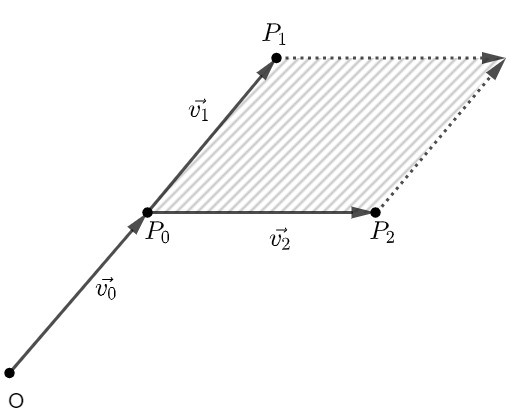
\includegraphics[width=.78\linewidth]{../figures/lec-25.1.png}
    \caption{Plane $\mathcal{S}$}
\end{wrapfigure}

Suppose $P_0,P_1,P_2$ be the points on $\R^3$ and coordinate vector of the points is given by,

\begin{align*}
    \vec{OP_0} & = \langle a_0,b_0,c_0 \rangle \\
    \vec{OP_1} & = \langle a_1,b_1,c_1 \rangle \\
    \vec{OP_2} & = \langle a_2,b_2,c_2 \rangle
\end{align*}

We will actually look at the parallelogram generated by,
\begin{align*}
    \vec{v_1} & = \vec{P_0P_1} \\
    \vec{v_2} & = \vec{P_0P_2}
\end{align*}

Any point inside the parallelogram must look like $\vec{v_0} + t_1 \vec{v_1} +t_2 \vec{v_2}$ for some $t_1,t_2 \in [0,1]$. So the parallelogram can be explicitly written as,

$$ \mathcal{S} = \{ \vec{v_0} + t_1 \vec{v_1} +t_2 \vec{v_2}  |  0 \le t_1,t_2 \le 1\} $$

We know area of $\mathcal{S}$ is $\norm{\vec{v_1}\times \vec{v_2}}$. We can describe this plane differently. If the equation of the plane was $z=ax+by+c$, then the surface of the plane can be described by $\mathcal{S} = \{(x, y, ax+by+c) | (x,y) \in B^2 \}$. Area of $\mathcal{S} = \sqrt{1+a^2+b^2} \times \text{Area}(B^2)$. Now we should move forward to the general case.

\begin{wrapfigure}{r}{0.50\textwidth}
    \centering
    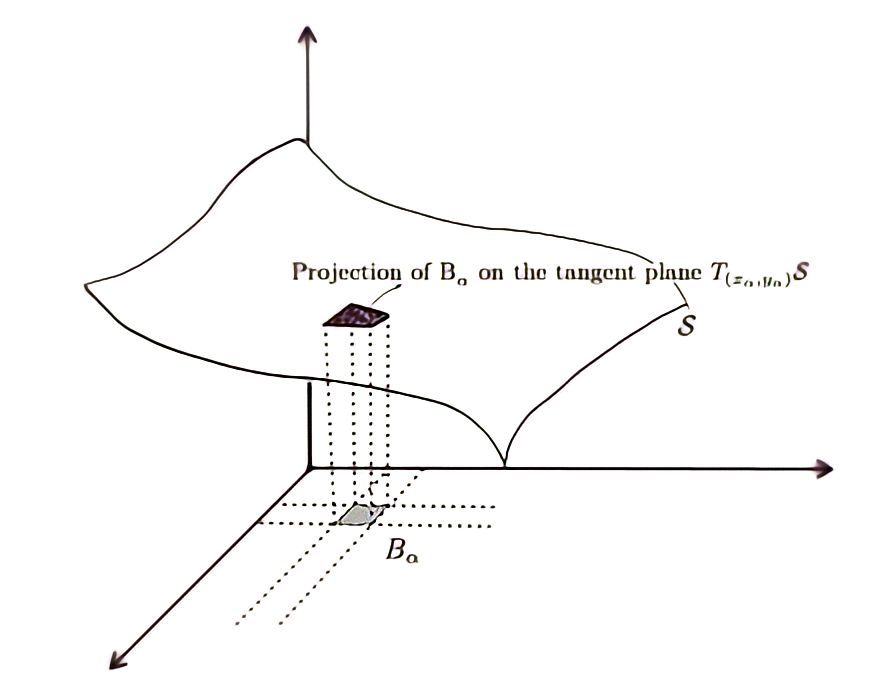
\includegraphics[width=.78\linewidth]{../figures/lec-25.2.png}
    \caption{$T_{r(x_{\alpha},y_{\alpha})} \mathcal{S}$}
\end{wrapfigure}


Let, $r : B^2 \to \R^3$ be a function defined as $r(x,y) = (x,y,f(x,y))$ (Here $f$ is $C^1$ function). Let, $\text{ran}(r)$ be the surface $\mathcal{S}$.

\vspace{0.2cm}

As we have done in the case of Riemann Integration. We should make partition of $B^2$ into tiny boxes.  Let, $\mathcal{P} \in \mathscr{P}(B^2)$. Then,
\[B = \bigcup_{\alpha \in \Lambda(\mathcal{P})} B_{\alpha}^2\]

For any $\alpha \in \Lambda(\mathcal{P})$ fix $(x_{\alpha},y_{\alpha}) \in B_{\alpha}^2$. Consider the tangent plane of $\mathcal{S}$ at $r((x_{\alpha},y_{\alpha}))$ over $B_{\alpha}^2$. Now the Tangent Plane at $r((x_{\alpha},y_{\alpha}))$ is given by,

\begin{align*}
    z - f((x_{\alpha},y_{\alpha})) & = (Df)(x_{\alpha},y_{\alpha}).(x_{\alpha},y_{\alpha})                                                                             \\
    \implies z                     & = (Df)(x_{\alpha},y_{\alpha}) + f(x_{\alpha},y_{\alpha})                                                                          \\
    \implies z                     & = f_X(x_{\alpha},y_{\alpha}) \cdot (x - x_{\alpha}) +f_Y(x_{\alpha},y_{\alpha}) \cdot (y - y_{\alpha}) + f(x_{\alpha},y_{\alpha}) \\
\end{align*}

So, Area of $T_{r(x_{\alpha},y_{\alpha})} \mathcal{S}$ over $B_{\alpha}^2$ is

$$\sqrt{1 + f_X^2(x_{\alpha},y_{\alpha}) + f_Y^2(x_{\alpha},y_{\alpha})} \times \text{Area}(B_{\alpha})^2$$

$$ = \norm{r_x \times r_y} \times \text{Area}(B_{\alpha})^2$$

\pagebreak

Since $f$ is $C^1$ function so is $r$. So the total area of the surface $\mathcal{S}$ is given by,

\begin{align*}
    \text{Area} (\mathcal{S}) & = \lim_{\norm{\mathcal{P}} \to 0} \norm{r_x \times r_y} \times \text{Area}(B_{\alpha})^2 \\
                              & = \int_{B^2} \norm{r_x \times r_y} dA                                                    \\
                              & = \int_{B^2} \sqrt{1 + f_X^2 +f_Y^2} \dd A \hspace{0.2cm}(\text{In this case})
\end{align*}

Will will do the above integration over any bounded set $\Omega$ as we have done in \text{Riemann} integration chapter. Over a bounded set $\Omega$ area of $\mathcal{S}$ is given by,

\[\text{Area} (\mathcal{S}) =  \int_{\Omega} \sqrt{1 + f_X^2 +f_Y^2} \dd A \label{eq:surfa} \cdots  (\ref{eq:surfa})\]

The General method for finding surface area is described by the following theorem.

\begin{Thm}{}{}
    Let $\mathcal{R} \subseteq \R^2$ be a region. $r : \mathcal{R} \to \R^3$ be the parametrization of the surface $\mathcal{S}$. Then,

    \[\text{Area}(\mathcal{S}) = \int_{\mathcal{R}} \norm{r_u \times r_v} \dd A\]
\end{Thm}

\end{document}